\documentclass[border=6pt,multi,tikz]{standalone}
\usepackage{tikz}
\usetikzlibrary{arrows.meta,positioning,fit,backgrounds,calc}

\definecolor{cSrc}{HTML}{E8F2E4}   \definecolor{cSrcB}{HTML}{6E9A68}
\definecolor{cQA}{HTML}{EDE6F5}    \definecolor{cQAB}{HTML}{8C74B5}
\definecolor{cSum}{HTML}{FDF3DC}   \definecolor{cSumB}{HTML}{C08F2E}
\definecolor{cGen}{HTML}{FCE6E2}   \definecolor{cGenB}{HTML}{BE6255}
\definecolor{cTrA}{HTML}{E0EFE7}   \definecolor{cTrAB}{HTML}{3A7350}
\definecolor{cTrB}{HTML}{FBE7D5}   \definecolor{cTrBB}{HTML}{BB7429}
\definecolor{cDet}{HTML}{E3EDF8}   \definecolor{cDetB}{HTML}{36669E}
\definecolor{cSco}{HTML}{FBF4D4}   \definecolor{cScoB}{HTML}{A8922A}
\definecolor{cJud}{HTML}{EEE9F6}   \definecolor{cJudB}{HTML}{73579F}
\definecolor{cHum}{HTML}{E2EFF1}   \definecolor{cHumB}{HTML}{2F7F86}
\definecolor{ink}{HTML}{1B2420}

\begin{document}
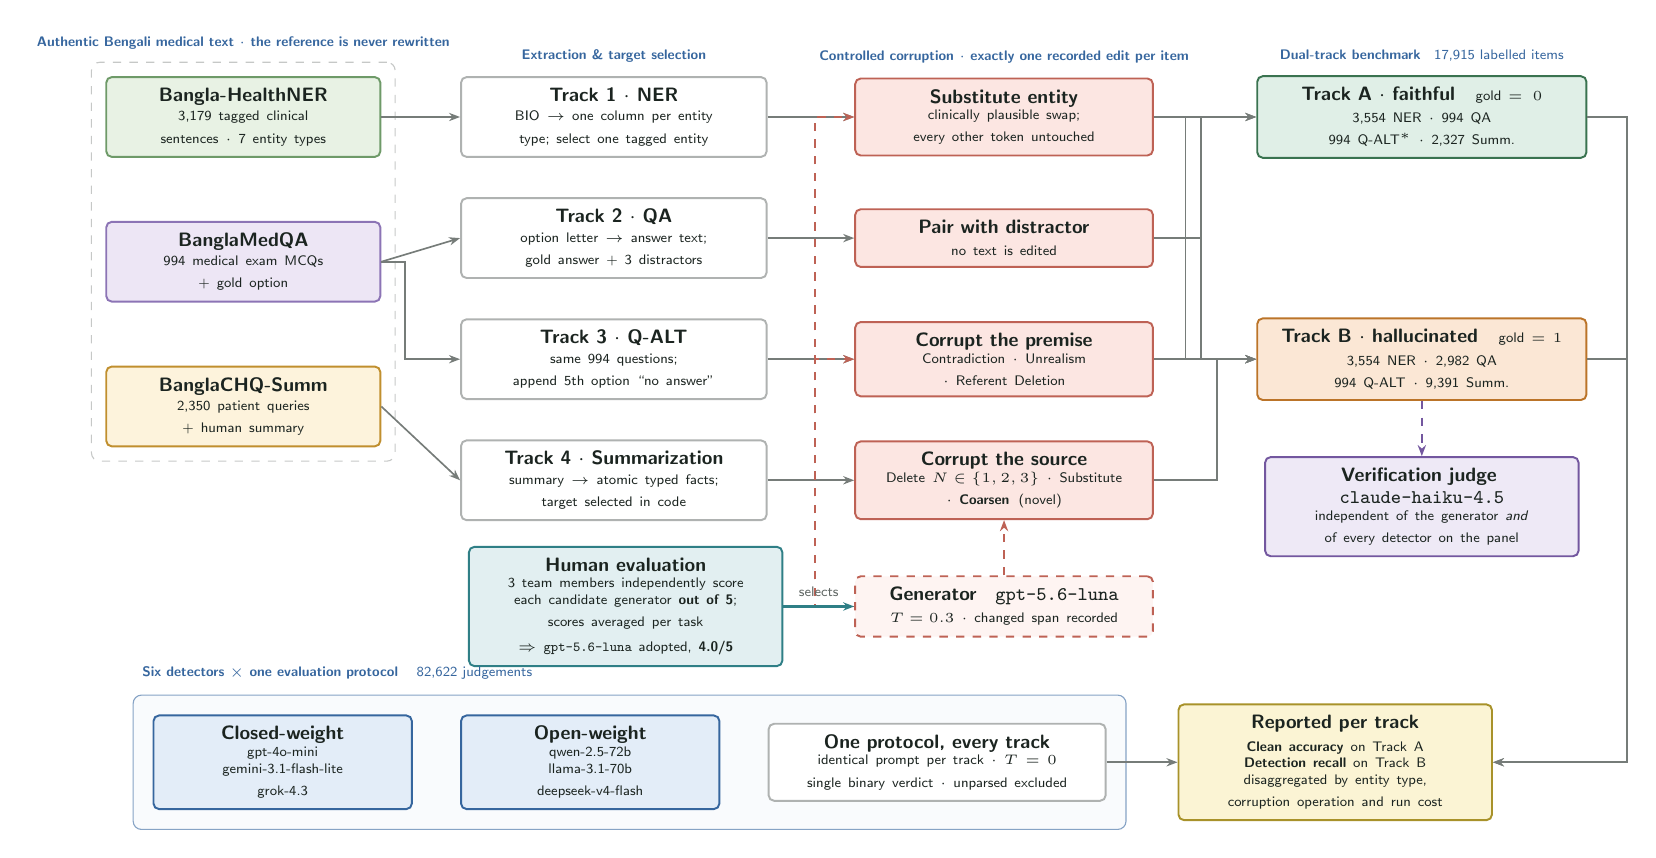
\begin{tikzpicture}[
  font=\sffamily\scriptsize, ink,
  box/.style={rounded corners=2pt,draw,line width=.7pt,align=center,inner sep=4pt},
  src/.style={box,fill=cSrc,draw=cSrcB,text width=32mm},
  qa/.style={box,fill=cQA,draw=cQAB,text width=32mm},
  sum/.style={box,fill=cSum,draw=cSumB,text width=32mm},
  stg/.style={box,fill=white,draw=ink!35,text width=36mm},
  op/.style={box,fill=cGen,draw=cGenB,text width=35mm},
  trk/.style={box,text width=39mm},
  det/.style={box,fill=cDet,draw=cDetB,text width=30mm},
  sco/.style={box,fill=cSco,draw=cScoB,text width=37mm},
  jud/.style={box,fill=cJud,draw=cJudB,text width=37mm},
  hum/.style={box,fill=cHum,draw=cHumB,text width=37mm},
  ar/.style={-{Stealth[length=4pt]},draw=ink!60,line width=.6pt},
  lbl/.style={font=\sffamily\tiny,ink!70},
  stage/.style={font=\sffamily\bfseries\tiny,cDetB},
]

%================ corpora
\node[src] (ner)  {\textbf{Bangla-HealthNER}\\[1pt]{\tiny 3,179 tagged clinical\\sentences $\cdot$ 7 entity types}};
\node[qa,below=8mm of ner] (mcq) {\textbf{BanglaMedQA}\\[1pt]{\tiny 994 medical exam MCQs\\+ gold option}};
\node[sum,below=8mm of mcq] (chq) {\textbf{BanglaCHQ-Summ}\\[1pt]{\tiny 2,350 patient queries\\+ human summary}};
\begin{scope}[on background layer]
  \node[draw=ink!25,dashed,rounded corners=3pt,fit=(ner)(mcq)(chq),inner sep=5pt] (corp) {};
\end{scope}
\node[stage,above=1pt of corp.north,anchor=south] {Authentic Bengali medical text $\cdot$ the reference is never rewritten};

%================ target selection
\node[stg,right=10mm of ner] (t1) {\textbf{Track 1 $\cdot$ NER}\\[1pt]{\tiny BIO $\rightarrow$ one column per entity\\type; select one tagged entity}};
\node[stg,below=5mm of t1] (t2) {\textbf{Track 2 $\cdot$ QA}\\[1pt]{\tiny option letter $\rightarrow$ answer text;\\gold answer + 3 distractors}};
\node[stg,below=5mm of t2] (t3) {\textbf{Track 3 $\cdot$ Q-ALT}\\[1pt]{\tiny same 994 questions;\\append 5th option ``no answer''}};
\node[stg,below=5mm of t3] (t4) {\textbf{Track 4 $\cdot$ Summarization}\\[1pt]{\tiny summary $\rightarrow$ atomic typed facts;\\target selected in code}};
\node[stage,above=1.5pt of t1.north,anchor=south] {Extraction \& target selection};

\draw[ar] (ner.east) -- (t1.west);
\draw[ar] (mcq.east) -- (t2.west);
\draw[ar] (mcq.east) -- ++(3mm,0) |- (t3.west);
\draw[ar] (chq.east) -- (t4.west);

%================ corruption
\node[op,right=11mm of t1] (o1) {\textbf{Substitute entity}\\{\tiny clinically plausible swap;\\every other token untouched}};
\node[op,right=11mm of t2] (o2) {\textbf{Pair with distractor}\\{\tiny no text is edited}};
\node[op,right=11mm of t3] (o3) {\textbf{Corrupt the premise}\\{\tiny Contradiction $\cdot$ Unrealism\\$\cdot$ Referent Deletion}};
\node[op,right=11mm of t4] (o4) {\textbf{Corrupt the source}\\{\tiny Delete $N\!\in\!\{1,2,3\}$ $\cdot$ Substitute\\$\cdot$ \textbf{Coarsen} \,(novel)}};
\node[stage,above=1.5pt of o1.north,anchor=south] {Controlled corruption $\cdot$ exactly one recorded edit per item};

\draw[ar] (t1) -- (o1);  \draw[ar] (t2) -- (o2);
\draw[ar] (t3) -- (o3);  \draw[ar] (t4) -- (o4);

\node[box,fill=cGen!45,draw=cGenB,dashed,text width=35mm,below=7mm of o4] (glm)
  {\textbf{Generator}\;\; \texttt{gpt-5.6-luna}\\{\tiny $T\!=\!0.3$ $\cdot$ changed span recorded}};
\draw[ar,dashed,draw=cGenB] (glm.north) -- (o4.south);
\draw[ar,dashed,draw=cGenB] (glm.west) -- ++(-5mm,0) |- (o3.west);
\draw[ar,dashed,draw=cGenB] (glm.west) -- ++(-5mm,0) |- (o1.west);

%================ human evaluation of the generators
\node[hum,left=9mm of glm] (hum)
 {\textbf{Human evaluation}\\{\tiny 3 team members independently score\\each candidate generator \textbf{out of 5};\\scores averaged per task}\\[1pt]
  {\tiny $\Rightarrow$ \texttt{gpt-5.6-luna} adopted, \textbf{4.0/5}}};
\draw[ar,draw=cHumB,line width=.8pt] (hum.east) -- node[lbl,above,pos=.5]{selects} (glm.west);

%================ tracks
\node[trk,fill=cTrA,draw=cTrAB,right=13mm of o1] (tA)
  {\textbf{Track A $\cdot$ faithful}\quad{\tiny gold $=0$}\\[2pt]
   {\tiny 3,554 NER $\cdot$ 994 QA\\994 Q-ALT$^{*}$ $\cdot$ 2,327 Summ.}};
\node[trk,fill=cTrB,draw=cTrBB,right=13mm of o3] (tB)
  {\textbf{Track B $\cdot$ hallucinated}\quad{\tiny gold $=1$}\\[2pt]
   {\tiny 3,554 NER $\cdot$ 2,982 QA\\994 Q-ALT $\cdot$ 9,391 Summ.}};
\node[stage,above=1.5pt of tA.north,anchor=south] {Dual-track benchmark \;\;{\mdseries 17,915 labelled items}};

\draw[ar] (o1.east) -- ++(4mm,0) |- (tA.west);
\draw[ar] (o2.east) -- ++(6mm,0) |- (tA.west);
\draw[ar] (o1.east) -- ++(4mm,0) |- (tB.west);
\draw[ar] (o2.east) -- ++(6mm,0) |- (tB.west);
\draw[ar] (o3.east) -- (tB.west);
\draw[ar] (o4.east) -- ++(8mm,0) |- (tB.west);

\node[jud,below=7mm of tB] (judge)
  {\textbf{Verification judge}\;\; \texttt{claude-haiku-4.5}\\{\tiny independent of the generator \emph{and}\\of every detector on the panel}};
\draw[ar,dashed,draw=cJudB] (tB.south) -- (judge.north);

%================ detection
\node[det] (d1) at ($(chq.south)+(5mm,-40mm)$) {\textbf{Closed-weight}\\{\tiny gpt-4o-mini\\gemini-3.1-flash-lite\\grok-4.3}};
\node[det,right=6mm of d1] (d2) {\textbf{Open-weight}\\{\tiny qwen-2.5-72b\\llama-3.1-70b\\deepseek-v4-flash}};
\node[box,fill=white,draw=ink!35,text width=40mm,right=6mm of d2] (prot)
  {\textbf{One protocol, every track}\\{\tiny identical prompt per track $\cdot$ $T\!=\!0$\\single binary verdict $\cdot$ unparsed excluded}};
\begin{scope}[on background layer]
  \node[draw=cDetB!60,rounded corners=3pt,fit=(d1)(d2)(prot),inner sep=7pt,fill=cDet!22] (detbox) {};
\end{scope}
\node[stage,anchor=south west] at ([yshift=2pt]detbox.north west)
  {Six detectors $\times$ one evaluation protocol \;\; \mdseries 82,622 judgements};

\node[sco,right=9mm of prot] (score)
  {\textbf{Reported per track}\\[2pt]
   {\tiny \textbf{Clean accuracy} on Track A\\
    \textbf{Detection recall} on Track B\\
    disaggregated by entity type,\\corruption operation and run cost}};

\draw[ar] (tA.east) -- ++(5mm,0) |- (score.east);
\draw[ar] (tB.east) -- ++(5mm,0) |- (score.east);
\draw[ar] (prot.east) -- (score.west);

\end{tikzpicture}
\end{document}
